\documentclass[11pt,a4paper, 
swedish,english %% Make sure to put the main language last!
]{article}
\pdfoutput=1

%% Andréas's custom package 
%% (Will work for most purposes, but is mainly focused on physics.)
\usepackage{../custom_as}

%% Figures can now be put in a folder: 
\graphicspath{ {figures/} %{some_folder_name/}
}

%% If you want to change the margins for just the captions
\usepackage[margin=10 pt]{caption}

%% To add todo-notes in the pdf
\usepackage[%disable  %%this will hide all notes
]{todonotes} 

%% Change the margin in the documents
\usepackage[
%            top    = 3cm,              %% top margin
%            bottom = 3cm,              %% bottom margin
%            left   = 3cm, right  = 3cm %% left and right margins
]{geometry}


%% If you want to chage the formating of the section headers
%\renewcommand{\thesection}{...}
\swapcommands{\Lambda}{\varLambda}
\swapcommands{\Omega}{\varOmega}
\swapcommands{\Gamma}{\varGamma}
\newcommand{\Lsq}[1]{\ensuremath{\mathcal{L}^2_{#1}}}
\newcommand{\RT}{\ensuremath{R_{\text{T}}}}
\newcommand{\RH}{\ensuremath{R_{\text{H}}}}
\newcommand{\tf}{\ensuremath{\tilde{f}}}

%%%%%%%%%%%%%%%%%%%%%%%%%%%%%%%%%%%%%%%%%%%%%%%%%%%%%%%%%%%%%%%%%%%%%%
\begin{document}%% v v v v v v v v v v v v v v v v v v v v v v v v v v
%%%%%%%%%%%%%%%%%%%%%%%%%%%%%%%%%%%%%%%%%%%%%%%%%%%%%%%%%%%%%%%%%%%%%%


%% If you want to use an external file for the title page
%\input{titlepages.tex}


%%%%%%%%%%%%%%%%%%%% vvv Internal title page vvv %%%%%%%%%%%%%%%%%%%%%
\begin{titlepage}
\title{\tt Project lambda}
\author{Niklas Renström \and Andréas Sundström}
\date{\today}

\maketitle

%% Page numbering:
%\pagenumbering{roman} %% roman pagenumbering
\thispagestyle{empty} \pagestyle{empty} %% no page numbers 

%% The abstract of the document
\begin{abstract} 


\end{abstract}
\newpage
\tableofcontents
\end{titlepage}

\pagenumbering{arabic}
\setcounter{page}{1}
%%%%%%%%%%%%%%%%%%%% ^^^ Internal title page ^^^ %%%%%%%%%%%%%%%%%%%%%
%% If you want a list of all todos
%\todolist


\section{Introduction}
%\todo[inline]{General intro to hyopthermia and freq dep.}

The current hyperthermia treatments mainly utilizes signals consisting of single or a narrow band (NB) of frequencies since simulations and numerical studies have not shown an increase of efficacy by using a wide band (WB). 
However, in mathematical theory there exists a number of uncertainty  principals stating that a function cannot be highly localized in the space and frequency domains at the same time which would encourage the use of a wide band of frequencies, in contrast to prior studies.

This project aims to shed some light to this apparent inconsistency by taking a closer look at relevant uncertainty principles and applying them to a simplified case of scalar fields satisfying the wave equation in two dimensions.
First the Heisenberg inequality, a lower limit of the product of the field's variance in the two domains in  will be applied.
Next, to get something more applicable to hyperthermia an uncertainty principle originally developed by D. Slepian, H.J. Landau and H.O. Pollak, which speaks of how well a function limited in frequency can be localized in a bounded region of space. At this point we will also introduce a polar wave decomposition to yield a more straight forward application of the theory than the normal plane wave decomposition.

Finally the results will be discussed from a hyperthermia treatment point of view and we will discuss some of the limitations as well as possible extensions of the theory.


\subsection{Limitations}
The human body contains many different materials and therefore a real hyperthermia treatment planning will often involve numerically solving Maxwell's equations to simulate how the EM-field will look like in the specific case.

Since this project aims to extract what limitations the wave \emph{nature} sets we are not concerned with the actual wave propagation -- instead we ask the question, given a perfect way to create or propogate the EM-field what limits does a narrow band of frequencies and the wave equation set on the optimal distribution in a bounded region?

With this in mind the study is limited to a homogeneous material stretching through all space. The material is assumed lossfree although the case of lossy materials and dampened EM-field's will be discussed briefly in chapter \ref{sec:discussion}.

Further we limit ourselves to 2 dimensions since this suffices to capture the essential wave nature (a circular ring of wavenumbers as opposed to a point in 1 dimension) whilst not overly complicating the mathematics. 
In this space we try to focus the distribution to a simple body, a disk since we believe that most more complicated bodies would yield approximately the same results.

We will also limit our attention to scalar fields, real EM-fields are in fact vectors with certain limitations to its directions which would produce slightly tighter bounds then what we achieved but this was unfortunately beyond the scope of this project.

Finally, for a real hyperthermia treatment it is not the intensity of the EM-field that is of concern but rather its mean-value in time that is of interest. This has major implications for the frequency dependence of the efficacy and will be discussed to some length in chapter \ref{sec:discussion}. However, the main part of this work is concerned with the EM-field itself and not its time mean.


\subsection{Theory}
For each frequency $\omega$ the electric field will have a harmonic timedependence,and can be represented by phasor notation,
\begin{equation}
  \label{eq:phasor}
\vb*E(\vb*x,t)=\Re\qty[\vb*E(\vb*x)\ee^{-\ii\omega t}]%\cos(\omega t).
\end{equation}
%which allows the use of phasors,
%\begin{equation}
%\vb*E(\vb*x,t)=\Re\qty[\vb*E(\vb*x)\ee^{-\ii\omega t}].
%\end{equation}
In a loss-less and source-less homogeneous media the Maxwell equations reduce to
\begin{equation}
\begin{cases}
\laplacian  \vb*E + k^2\vb*E=0,\\
\div\vb*E = 0,
\end{cases}
\end{equation} 
where $k^2 = \omega^2/v^2$ with $v=\frac{1}{\sqrt{\mu \epsilon}}$ being the speed of propagation. 

To simplify matters however, we will limit the scope of this project to scalar fields satisfying the Helmholtz equation
\begin{equation}
  \label{eq:Helmholtz}
  \qty(\laplacian + k^2)E=0.
\end{equation} 

\subsubsection{Plane wave decomposition}
One solution to the Helmoholtz equation \eqref{eq:Helmholtz} are the plane waves
\begin{equation}\label{eq:plane-wave}
E(\vb*x)=A \ee^{\ii\vb*k \cdot \vb*x},
\end{equation}
were the wavevector $\vb*k$ is any vector such that $\vb*k\vdot\vb*k=k^2$, and $A$ is a constant amplitude. 

The next step is to allow more for more than one frequency. The solution for each frequency will be of the form \eqref{eq:plane-wave}, each with its own amplitude $A(\vb*k)$. These solutions can then be summed up over all frequencies (magnitude as well as directions of $\vb*k$) and the final $E$ field becomes\footnotemark{}
\begin{equation} \label{eq:FT-inv}
E(\vb*x)= (2\pi)^{-D} \oldint_{\vb*k} \rd^Dk\,
A(\vb*k) \ee^{\ii\vb*k\vdot\vb*x}.
\end{equation}
\footnotetext{The factor of $(2\pi)^{-D}$ is just for convenience in the comparison with the $D$ dimensional Fourier transform.}

We can now identify \eqref{eq:FT-inv} as an inverse Fourier transform
of $A(\vb*k)$, and thus $A(\vb*k)$ has to be the Fourier transform of
$E(\vb*x)$:
\begin{equation}\label{eq:FT}
A(\vb*k) = \oldint_{\vb*x} \rd^Dx\, E(\vb*x)\ee^{-\ii \vb*k\vdot\vb*x}.
\end{equation}


\subsubsection{Polar wave decomposition in 2 dimensions}
The 2 dimensional Helmholtz equation \eqref{eq:Helmholtz} in polar cooridnats is
\begin{equation}
\label{eq:Helmholtz_polar}
\qty(\pdv[2]{r}+\frac{1}{r}\pdv{r}+\frac{1}{r^2}\pdv[2]{\theta})E+k^2E=0,
\end{equation} 
Which has the standard non-singular solution
\begin{equation}
E(r, \theta)=\sum_{n=-\infty}^{\infty} a_nJ_n(kr)\ee^{\ii n \theta}.
\end{equation}

Analogously to the plane wave decomposition, we now introduce a spectrum of frequencies, and obtain
\begin{equation}
\label{eq:polar_wave_general}
E(r,\theta)
=\oldint_{k} \rd k \sum_{n=-\infty}^{\infty}\!\!a_n(k) J_n(kr)\ee^{\ii n \theta}
=\sum_{n=-\infty}^{\infty}\!\! \ee^{\ii n \theta} \oldint_{k} \rd{k}\,k\,b_n(k) J_n(kr),
\end{equation}
where in the last step $a_n(k)$ has been replaced with $k\,b_n(k)$ for later convenience.

%\subsubsection{Connection between Fourier and Bessel decomposition}





\section{Localization measures}
To start talking about focusing waves, one has to be able 
to quantify how localized it is. This is mainly done through
different measures on the energy distribution of the wave,
$\abs{f}^2$. 

This report will mainly deal with the fraction of energy in a bounded
area, which was used by
Slepian, Pollack and Landau (SPL) in a series of papers 
\cite{PSWF-I_1961,PSWF-II_1961,PSWF-III_1962,PSWF-IV_1964,PSWF-V_1978}.
However, to address the Heisenberg uncertainty principle, which
concerns a type of variance measure, an account of both types of
measures and how they are used will be given in this section. 


\subsection{Heisenberg's uncertainty principle}
The common quantum mechanical version of Heisenberg's uncertainty
principle states that \emph{the product of the variance of
  position and momentum must be greater than some fixed value}. This
is rooted in the interpretation that position and momentum are
related through fourier transfrom. 

The general mathematical statement of the Heisenberg uncertainty
principle, for a function $f$ and its Fourier transfrom\footnotemark{}
$\tf$, is \cite{Folland} 
\footnotetext{With the Fourier transform defined as in \eqref{eq:FT}. }
\begin{equation}
\Delta_{\vb*a}f \Delta_{\vb*\alpha} \tf \geq \frac{D^2}{4} \quad 
%\forall \vb*a, \vb*\alpha, 
\forall f \in \Lsq{\infty},%[\mathbb{R}^2],
\end{equation}
where $\Delta_{\vb*a}f$ is a variance measure of $f$ is around
\emph{any} reference point $\vb*a$, analogously for
$\Delta_{\vb*\alpha}\tf$ and $\vb*\alpha$.
These variances are defined by
\begin{equation} \label{eq:spread_def}
\Delta_{\vb*a}f=
\frac{\oldint_{\vb*x}\rd^Dx\,\abs{\vb*x-\vb*a}^2\abs{f(\vb*x)}^2}
{\oldint_{\vb*x}\rd^Dx\,\abs{f(\vb*x)}^2},
\end{equation}
and analogously for the Fourier transfrom.
% The minimum is achieved when $\vb*a$ ($\vb*\alpha$) is at the center
% of mass of $f$ ($\tf$):
% \begin{equation}
% \vb*x_{\text{CM}}=\frac{\oldint_{\vb*x}\rd^Dx\,\vb*x\abs{f(\vb*x)}^2}
% {\oldint_{\vb*x}\rd^Dx\,\abs{f(\vb*x)}^2}.
% \end{equation}


If $\Delta_{\vb*a}f$ is high, $f$ cannot be highly localized to one
single small neighbourhood in space. It does not however, preclude $f$
from having narrow peaks; there can exist several narrow peaks which
are spread out from each other and still have $\Delta_{\vb*a}{f}$
being large. 
For hyperthermia treatment, this means that the variation measure at
best gives a hint on what we want. It is possilbe to achieve a very
strong and narrow radiation peak inside the tumour without violating
the Heisenberg inequality, i.e. using NB signals, as long as a
significant part of the radiation intensity is located outside of the 
head.  
This is a consequence of the particular localization measure used in
the Heisenberg uncertainty relation. It is still a mathematical truth,
but it might be too blunt to be practically applicable in hyperthermia
treatments. 



\subsection{The Slepian-Pollack-Landau method}
\label{sec:SPL-method}
Another localization measure was used by SPL in
\cite{PSWF-I_1961,PSWF-II_1961,PSWF-III_1962,PSWF-IV_1964,PSWF-V_1978}. 
\todo{Maybe change?}
In what follows we will show the broad strokes for developing this
theory. In doing so we will prove the existance of a useful set of
functions ${\psi_i}$ which span the room of frequency-limited
functions.%  and one of which maximizes the energy retained for a
% frequency-limited function also limited in the space $S$. 

A square-integrable function $f$ of $D$ variables is said to be
$\Omega$-limited if it can be represented as a Fourier integral over
the bounded region $\Omega$, 
\begin{equation}\label{eq:freq-lim}
f(\vb*x)=\qty(2\pi)^{-D}\oldint_\Omega \rd^Dk\,
\tf(\vb*k)\ee^{\ii(\vb*k \cdot \vb*x)} 
\end{equation}
i.e. it only contains frequencies in the area $\Omega$.

% The total energy of a function is defined as
% \begin{equation*}
% A=\oldint_{R^D}\abs{f(\vb*x)}^2\id^Dx
% =\qty(\frac{1}{2\pi})^D \oldint_\Omega \abs{\tf(\vb*k)}^2\id^Dk,
% \end{equation*}
% where the last equality is due to Parseval.

The energy of a function $f$ in a region $S$ is defined as 
\begin{equation}\label{eq:AS}
A_S=\oldint_S\rd^Dx\,\abs{f(\vb*x)}^2.
\end{equation}
Using Parseval's formula, the total engergy of the $\Omega$-limited
function $f$ can be written as 
\begin{equation}\label{eq:Atot}
A=\oldint_{R^D}\rd^Dx\, \abs{f(\vb*x)}^2 =
(2\pi)^{-D}\oldint_\Omega\rd^Dk\, \abs{\tf(\vb*k)}^2.
\end{equation}


By substituing \eqref{eq:freq-lim} into \eqref{eq:AS}, we get
\begin{equation}\label{eq:AS-KS}
\begin{aligned}
A_S%=\oldint_S\abs{f(\vb*x)}^2\id^Dx
&=\qty({2\pi})^{-2D} \oldint_S\rd^Dx \oldint_\Omega \rd^Dk\,
\tf(\vb*k)\ee^{\ii\vb*k\cdot \vb*x}
\oldint_\Omega \id^Dk'\,
\tf^*(\vb*k')\ee^{-\ii\vb*k'\cdot \vb*x}\\
&=\qty (2\pi)^{-D} \oldint_\Omega\rd^Dk\oldint_\Omega\rd^Dk'\,
\tf(\vb*k)\tf^*(\vb*k')K_s(\vb*k-\vb*k')\\
%&=\ip{I\tf}{\tf}
\end{aligned}
\end{equation}
where
\begin{equation} \label{eq:kernel}
K_s(\vb*k-\vb*k')=(2\pi)^{-D}\oldint_S\rd^Dx\,
\ee^{\ii\vb*x \cdot(\vb*k-\vb*k')},
\end{equation}
is called an integral \emph{kernel}.
Define an integral operator $I_S$:
\begin{equation} \label{eq:int_op}
\qty[I_S g](\vb*k')=\oldint_\Omega\rd^Dk\, 
K_S(\vb*k-\vb*k')g(\vb*k).
\end{equation}
The fraction of energy that the $\Omega$-limited function $f$ can have
in a region $S$ can then be written as 
\begin{equation} \label{eq:energy_frac_final}
\frac{A_s}{A}=
\frac{\oldint_\Omega\rd^Dk\, \qty[I\tf](\vb*k)\tf^*(\vb*k)}
{\oldint_\Omega \rd^Dk\, \abs{\tf(\vb*k)}^2}
=\frac{\ip{I_S\tf}{\tf}}{\ip{\tf}},
\end{equation}
where we have defined an inner product on the $\Omega$-space:
\begin{equation} \label{eq:in_prod}
\ip{f}{g} =\oldint_\Omega\rd^Dk\, f(\vb*k)g^*(\vb*k).
\end{equation}

% In the litterature integral operators, like \eqref{eq:int_op},
% are called Hilbert-Schmidt integral operators if the kernel is
% square-integrable in $\Omega$, and such an operator is compact. 
% Since the regions $S$ and $\Omega$ are bounded square-integrability
% holds for the kernel \eqref{eq:kernel} and since it is also complex
% symmetric with respect to its arguments,
% $K_s(\vb*k-\vb*k')=K_s^*(\vb*k'-\vb*k)$, the integral operator 
\todo{CITE!}
It can be shown that the integral operator \eqref{eq:int_op} is 
self-adjoint and compact. From the Spectral theorem it now follows
that the functions fullfilling the eigenvalue equation 
\begin{equation}
  \label{eq:eigen}
\qty[I_S\psi](\vb*k)=\oldint_\Omega \rd^Dk'\,K_s(\vb*k')\psi(\vb*k') 
=\mu \psi(\vb*k)
\end{equation}
form an orthogonal base for the space $\Omega$. 
It also follows that the maximum of equation
\eqref{eq:energy_frac_final} is
the largest eigenvalue $\mu_0$ of equation \eqref{eq:eigen}. In
other word $\mu_0$ is an upper bound for the fraction of erergy
in $S$ for an $\Omega$-limited function. 
This upper bound will be dependent on the geometries of the areas
$S$ and $\Omega$. The following section will be devoted to calculating
this $\mu_0$ for bandwidth limited function in two dimensions. 



\section{Two dimensional application to
 signals of limited bandwidth}
%For the EM-field this gives an inequality for each component $E_i$\footnotemark{}
%\begin{equation}
%  \label{eq:ineq_final}
%  \Delta_{\vb*a}E_i\geq \frac{9}{4} \frac{1}{\mathrm{Min}_\alpha\Delta_{\vb*\alpha}\tilde{E_i}}, \quad \forall \vb*a.
%\end{equation}
\todo[inline]{Need to rewrite! Or move?}
Since the fourier transform of the EM field is concentrated on a sphere we achieve the minimum spread for $\alpha=0$ and using equations \eqref{eq:spread_def} one gets,
$\min_\alpha\Delta_{\vb*\alpha}\tilde{E}=\frac{\omega^2}{v^2}$ and \eqref{eq:ineq_final} becomes
\begin{equation}
 \Delta_{\vb*a}E\geq \frac{9v^2}{4\omega^2}=\frac{9\mu^2}{16\pi^2}=\frac{9}{16\pi^2\epsilon\mu\nu^2}.
 \end{equation}
\todo[inline]{end}

\todo[inline]{REDO intro}
So far we have looked at areas in the space and frequency domains
which have the same shape, filled discs or spheres, but are scaled
versions of each other ($S=c\Omega$). This corresponds to
including frequencies all the way down to 0, which is not an ideal
description of a real hyperthermia system which perhaps operates in the
range from few hundered MHz up to a couple of GHz.

The areas $S$ and $\Omega$ in the space respectively frequency domain have to
be defined separately.
For the space domain we still want a
filled region without a gap in the center, but for the frequency domain
we want to exclude the center part of the region.
Therefore, we let $S$ be a filled
circle disc of radius $R$, and $\Omega$ be the finite thickness circle
ring with outer radius $\Gamma$ and inner radius $q\Gamma$, $0\le q<1$.


\subsection{The SPL method using Fourier transforms}
%\todo[inline]{Move most of the math here to appendix!}
The methodology used here is a direct translation of the ones used in
\cite{PSWF-I_1961} and \cite{PSWF-IV_1964} to $S$ and $\Omega$. This
section will be somewhat short and superficial; this is due to the
fact that the next method will be much more efficient
numerically. Althogh there are some useful tools which will be
developed here.


From the definition of the kernel $K_s$ in equation \eqref{eq:kernel}, we get 
\begin{equation}
K_S(\vb*k-\vb*k') = (2\pi)^{-2}
\oldint_S \rd^2r \ee^{\ii\vb*r\vdot(\vb*k-\vb*k')}.
\end{equation}
By substituting to polar coordinates and using the usual Bessel
function expansion \cite[formula 8.551.4b]{Gradshteyn-Ryzhik} 
\begin{equation}
\ee^{\ii z\cos\theta} = \sum_{m=-\infty}^\infty
\ii^mJ_m(z)\ee^{\ii m\theta}
\end{equation}
and some other Bessel function identities 
\cite[formula~8.472.3]{Gradshteyn-Ryzhik}, we eventually end up with
\begin{equation}\label{eq:KS-short}
K_S(\vb*k-\vb*k') 
=(2\pi)^{-1}R\, \frac{J_1(R\Delta{k})}{\Delta{k}}.
\end{equation}
With the law of cosines
$\Delta{k}=\abs{\vb*k-\vb*k'}=\sqrt{k^2+{k'}^2-2kk'\cos(\Delta\theta)}$,
where $k=\abs{\vb*k}$, $k'=\abs{\vb*k'}$ and
$\Delta\theta=(\theta-\theta')$ is the angle between $\vb*k$ and
$\vb*k'$.

The numerical method described in Appendix~\ref{apx:num} can only be
applied to 1 dimensional integrals.
To reduce the eigenvalue equation \eqref{eq:eigen} to this form, first
note that $K_S(\vb*k-\vb*k')$ is $2\pi$-periodic in $\Delta\theta$,
and thus has a Fourier series expansion  
\begin{equation} \label{eq:KS-FS}
K_S(k, k', \Delta\theta)  
=\sum_{n=-\infty}^\infty a_{n}(k, k')\, \ee^{\ii n\Delta\theta}
=\sum_{n=-\infty}^\infty \ee^{\ii n\theta}\,a_{n}(k, k')\,\ee^{-\ii n\theta'},
\end{equation}
where 
\begin{equation} \label{eq:KS-FS-coef}
a_{n}(k, k') = \frac{1}{2\pi} \int_0^{2\pi} \rd(\Delta\theta)\; 
K_S(k, k', \Delta\theta)\ee^{-\ii n\Delta\theta}.
\end{equation}
Viewing \eqref{eq:eigen} as the definition of $\psi$, we also know
that the eigenfunctions, $\psi$, has to be periodic in 
$\theta$ since the kernel is periodic in $\theta$. Therefore
$\psi(k, \theta)$ also has to have a Fourier series 
\begin{equation}\label{eq:psi-FS}
\psi(k, \theta) = \sum_{m=-\infty}^\infty b_m(k)\ee^{\ii m\theta}.
\end{equation}
Substituting \eqref{eq:KS-FS} and \eqref{eq:psi-FS} into
\eqref{eq:eigen}, using polar coordinates and changing the order of
summation and integration, yields
\begin{equation}
\mu\sum_{l=-\infty}^\infty b_l(k)\ee^{\ii l\theta}
= \sum_{n=-\infty}^\infty \ee^{\ii n\theta} \sum_{m=-\infty}^\infty 
\int_{q\Gamma}^\Gamma\rd{k'}\,k' a_n(k, k') b_m(k')
\int_{0}^{2\pi}\rd\theta'\,
\ee^{\ii (m-n)\theta'}.
\end{equation}
The $\theta'$ integral is only non-zero when $(m-n)=0$ and
then the integral is just $2\pi$. We now get
\begin{equation}
\mu\sum_{l=-\infty}^\infty b_l(k)\ee^{\ii l\theta}
= 2\pi\sum_{n=-\infty}^\infty \ee^{\ii n\theta} 
\int_{q\Gamma}^\Gamma\rd{k'}\,k' a_n(k, k') b_n(k').
\end{equation}
By the uniqueness of Fourier series expansions, for all non-zero $b_n$
we finally obtain a one dimensional eigenvalue equation
\begin{equation}
\label{eq:eigen_fourier_coef}
\mu_n b_n(k) = 2\pi\int_{q\Gamma}^\Gamma\rd{k'}\,k' a_n(k, k') b_n(k'),
\end{equation}
where $\mu$ has been denoted by $\mu_n$ since each $b_n(k)$
will have a different eigenvalue satisfying
\eqref{eq:eigen_fourier_coef}.  

There is one last thing we can do to make
\eqref{eq:eigen_fourier_coef} more suitable for numerical solution,
and that is to symmetrisize the kernel $k'a_n(k, k')$. To do that we
make the substitution $b_n(k)=\phi_n(k)/\sqrt{k}$, which yields
\begin{equation}
\mu_n \phi_n(k) = 2\pi\int_{q\Gamma}^\Gamma\rd{k'}\,
\sqrt{kk'}a_n(k, k') \phi_n(k').
\end{equation}
This makes the kernel $\sqrt{kk'}b_n(k, k')$ symmetric in $k$ and
$k'$, since $b_n(k, k')=b_n(k', k)$ was already symmetric. Besides
making the numerical eigenvalue calculation more efficient, this also
has some nice mathematical implications. Like for instance $\phi_n$
constituting an orthogonal base on $[q\Gamma, \Gamma]$.\todo{cite!}

However, the problem with this method is that the Fourier coefficients
of the kernel, $b_n(k, k')$, cannot be calculated analytically by
direct integration using standard methods. This results in very costly
numerical calculations since $b_n(k, k')$ has to be calculated
numerically for each pair of $k$ and $k'$, on top of then calculationg
the eigenvalues. 
This problem stems from trying to adobt a plane wave decomposition to
polar coordinates. By starting from the polar wave decomposition one
can avoid these difficulties, which is what we will do in the
following section. 


\subsection{Expanding the SPL method using Bessel decomposition}
The SPL method can be expanded to also cover polar decomposition
\eqref{eq:polar_wave_general}. The main idea of this generalization is
that for circularly symmetric geometries in 2D, polar decomposition
using Bessel function is more natural. 
This generalization will here be illustrated through the example using
$S$ and $\Omega$ as defined above, and the goal should be to
circumvent the problem of evaluating \eqref{eq:KS-FS-coef} from the
previous section.

To calculate the energy of the field $E$ in the disk $S$, we
substitute \eqref{eq:polar_wave_general} into \eqref{eq:AS}: 
\begin{equation}
\begin{aligned}
A_S= \int_S \rd^2x\, \abs{E}^2 = 
\int_0^{R_S} r\rd{r} \int_0^{2\pi} \rd\theta \,&
\int_{q\Gamma}^\Gamma \rd{k}\!\!
\sum_{n= -\infty}^{\infty}\!\! kb_n(k) J_n(kr)\ee^{\ii n \theta}\\
&\times
\int_{q\Gamma}^\Gamma \rd{k'}\!\!
\sum_{m= -\infty}^{\infty}\!\! k'b_m^*(k') J_n(k'r)\ee^{-\ii m
  \theta}.
\end{aligned}
\end{equation}
If we now rearrange the order of sumation and integration, and
evaluate the $\theta$ integral, we see that non-vanishing terms are
with $m=n$ and then we get a factor of $2\pi$ like in the previous
section. By introducing the kernel 
\begin{equation}\label{eq:KS-bessel}
K_S^{(n)}(k, k') = \int_{0}^{R_s} \rd{r}\, r J_n(kr) J_n(k'r),
\end{equation}
the energy in $S$ can be written as
\begin{equation}\label{eq:AS-bessel}
A_S =2\pi \sum_{n=-\infty}^{\infty} 
\int_{q\Gamma}^\Gamma \rd{k} \int_{q\Gamma}^\Gamma \rd{k'}\,  
kk'\, b_n(k)b_n^*(k') K_S^{(n)}(k, k')
\end{equation}

If we let the radius $R_S$ of the disk $S$ tend to infinity, and by
using the asymptotic behavior of Bessel functions, the the infinte
kernel can be witten as\todo{cite, Arfken-Weber?}
\begin{equation}
K_\infty^{(n)}(k,k') = \frac{\delta(k-k')}{k'}.
\end{equation}
This implies that the total energy
\begin{equation}\label{eq:A-bessel}
\begin{aligned}
A &=2\pi \sum_{n=-\infty}^{\infty} 
\int_{q\Gamma}^\Gamma \rd{k} \int_{q\Gamma}^\Gamma \rd{k'}\,  
kk'\, b_n(k)b_n^*(k') \frac{\delta(k-k')}{k'} \\
&=2\pi \sum_{n=-\infty}^{\infty} 
\int_{q\Gamma}^\Gamma \rd{k} \, k\, b_n(k)b_n^*(k).
\end{aligned}
\end{equation}

With \eqref{eq:AS-bessel} and \eqref{eq:A-bessel}, the energy fraction
can be written as
\begin{equation}\label{eq:E-frac-bessel}
\frac{A_S}{A}
=\frac{\displaystyle{\sum_{m}} \int_{q\Gamma}^\Gamma \rd{k} \int_{q\Gamma}^\Gamma \rd{k'}\,  
kk'\, b_m(k)b_m^*(k') K_S^{(m)}(k, k')}
{\displaystyle{\sum_{n}} \int_{q\Gamma}^\Gamma \rd{k} \, k\, b_n(k)b_n^*(k)}.
\end{equation}
By similar arguments as in Section~\ref{sec:SPL-method}, the maximum
of this fraction is given as the largest eigenvalue to
\begin{equation}
\mu_nb_n(k) = \int_{q\Gamma}^{\Gamma}\rd{k}\,k K_S^{(n)}(k, k')\,b_n(k').
\end{equation}
Note that the equation above is different for each $n$, and the
maximum is to be taken over all $n$.

Analagously to the case in the previons section, theis eigenvalue
equation can be symmetrisized to
\begin{equation}
\mu_n\phi_n(k) = \int_{q\Gamma}^{\Gamma}\rd{k}\,
\sqrt{kk'} K_S^{(n)}(k, k')\,\phi_n(k').
\end{equation}
\todo[inline]{Equivalence!}

The advantage of this method is that this time, the kernel
\eqref{eq:KS-bessel} can be calculated analytically
\cite[Formula 5.54]{Gradshteyn-Ryzhik}
\begin{equation}
K_S^{(n)}(k, k') =
\begin{cases}
\frac{R_S}{k^2-k'^2}
\qty[k'J_{n}(R_sk)J_{n-1}(R_sk')-kJ_{n-1}(R_sk)J_{n}(R_sk')]
\qc &k\neq k'\\
\frac{R_S^2}{2}\qty[ \qty(J_{n}(R_Sk))^2
-J_{n-1}(R_sk)J_{n+1}(R_sk)]
\qc &k= k'.
\end{cases}
\end{equation}
So now, the numerical calculation of the eigenvalues are significantly
faster than with the previous method.

\section{SAR}

\newtheorem{theorem}{Theorem}
In hyperthermia treatment a good indicator for the temperature
increase is the Specific Absorbation Rate (SAR): 
\begin{equation*}
\text{SAR}(\vb*x)=
\frac{\ev{\vb*J(\vb*x,t)\vdot \vb*E(\vb*x,t)}_t}{\rho(\vb*x)},
\end{equation*}
where $\vb*J$ is the current density, $\vb*E$ is the
electric field, $\rho$ is the mass density, and $\ev{\xi}_t$ denotes
the time average of some quantity $\xi$.
Due to Ohm's law this is simply a weighted version of the intensity
$I=\abs{\vb*E}^2$.
However, due to the time-averaging intereference between multiple
frequencies vanishes. Thus
\begin{equation}
\text{SAR}(\vb*x)=\sum_i\text{SAR}_{\omega_i}(\vb*x),
\end{equation}
that is a sum over the contribution from each frequency.
% In other words, when time-averaging there is no interference between different frequencies.

Since a finite energy will always be applied, all possible solutions
will be a convex combination of the contribution for each
frequency. And due to the linearity over frequencies, any convex
goalfunction $G(\text{SAR})$ will be convex in the frequencies and a
powerful theorem from convex optimization can be applied: 
\begin{theorem}
 Let $f$ be a convex function defined on a convex set $X$. Then any
 local minima of $f$ is also a global minima on $X$. 
\end{theorem}
This implies that the minimum of $G$ is obtained with only the
frequency $\omega_j$ that gives the smallest contribution to $G$. 

For a large family of goalfunctions the optimum is therefore obtained
for a single frequency. In particular, any linear goalfunction is also
convex and the main goalfunction used in this paper,
\eqref{eq:energy_frac_final} would be optimized\footnote{the inverse
  of it would be minimized} by a single frequency if applied to SAR.  

\todo[inline]{Expression for single frequency}

%%%%%%%%%%%%%%%%%%%%%%%%%%%%%%%%%%%%%%%%%%%%%%%%%%%%%%%%%%%%%%%%%%%%%%
\section{Results}

\begin{figure}\centering
\centerline{ % centers figures larges than 1\textwidth
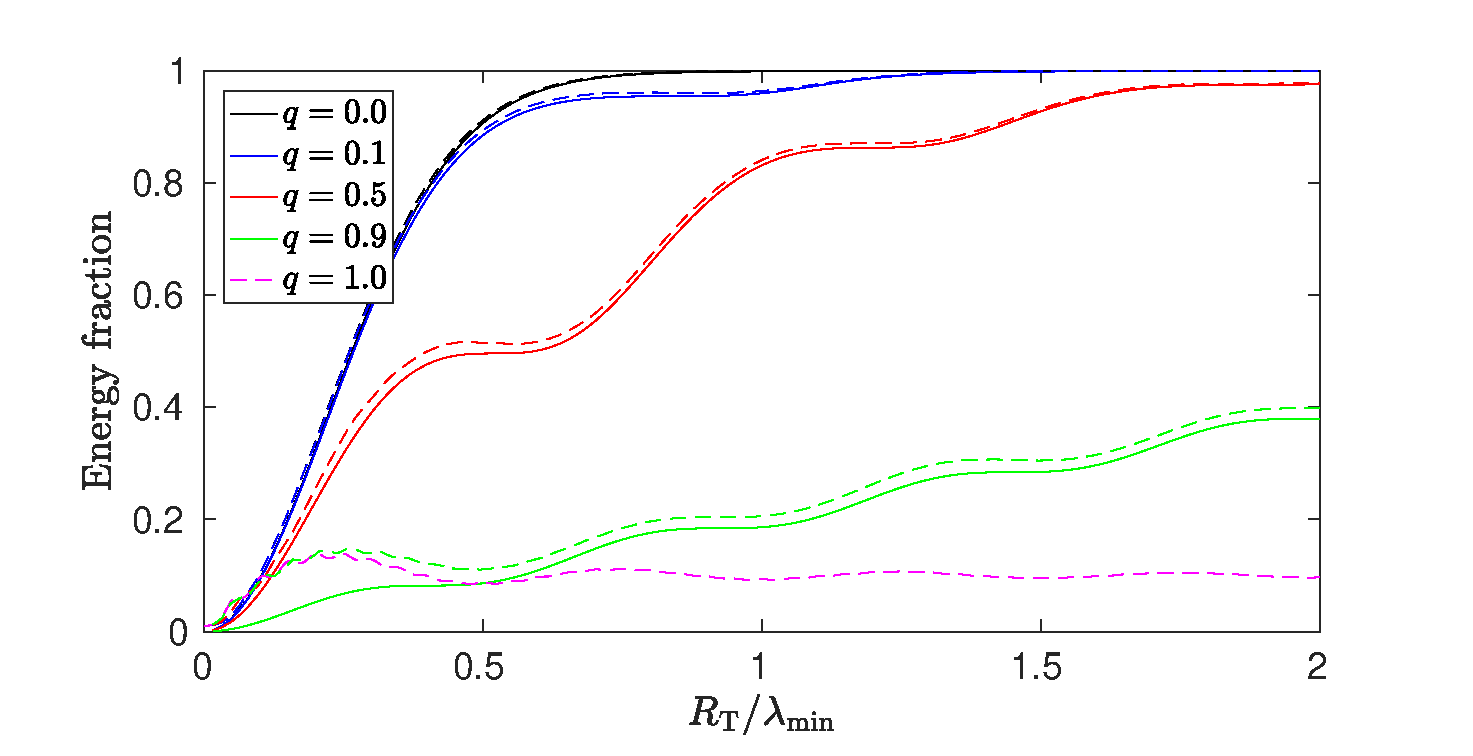
\includegraphics[width=18cm]{ring_both_L1000.eps}
}
\caption{Theoretical maximum of energy fraction inside the tumor, both
  compared to the total energy in real space (line) as well as
  compared to a ``head'' region (dashed). The fraction are plotted as
  a function of tumor size, $\RT$, measured in sortest wavelengths,
  $\lambda_{\min}$. The different values of $q$ corresponds to the width of
  the frequency band, where $\lambda_{\min}=\RT/(2\pi c)$ and
  $\lambda_{\max}=\RT/(q2\pi c)=\lambda_{\min}/q$, i.e. a larger $q$
  means a narrower band. }
\label{fig:both}
\end{figure}


%%%%%%%%%%%%%%%%%%%%%%%%%%%%%%%%%%%%%%%%%%%%%%%%%%%%%%%%%%%%%%%%%%%%%%
\section{Discussion and outlooks}
\label{sec:discussion}


%%%%%%%%%%%%%%%%%%%%%%%%%%%%%%%%%%%%%%%%%%%%%%%%%%%%%%%%%%%%%%%%%%%%%%
\section{Conclusions}





%%%%%%%%%%%%%%%%%%%%%%%%%% The bibliography %%%%%%%%%%%%%%%%%%%%%%%%%%
%\newpage
%% This bibliography ueses BibTeX
\bibliographystyle{ieeetr}
\bibliography{references}%requires a file named 'references.bib'
%% Citations are as usual: \cite{example_article}

%%%%%%%%%%%%%%%%%%%%%%%%%%%%% Appendices %%%%%%%%%%%%%%%%%%%%%%%%%%%%%
\clearpage %% on a new page 
\appendix  %% This will change the page numbering to A1, A2, A3, ...;
           %% and also change the sections to A, A.1, ...; B, B.1, ...


%%%%%%%%%%%%%%%%%%%%%%%%%%%%%%%%%%%%%%%%%%%%%%%%%%%%%%%%%%%%%%%%%%%%%%
\section{Numerical implementation of the 
Landau-Pollack-Slepian Theory}
\label{apx:num}
In the previous section we have been occupied by integral eigenvalue
equations of the form
\begin{equation} %\label{eq:int-eig}
\mu E(k) 
= \oldint_{\Omega} \rd^D{k}\, K(k, k') E(k')
\qcomma k, k'\in\Omega.
\end{equation}
We have also put down some work to reduce higher-dimensional
integrals to one-dimensional ones
\begin{equation} \label{eq:int-eig}
\mu \psi(k) 
= \oldint_{I} \rd{k}\, K(k, k') \psi(k'),
\end{equation}
where the integration is now over an interval 
$I=[\alpha, \beta]$. This was done so that the numerical method
presented here could be applied. 


\subsection{Discretization of the integral equation}
The integral can be discretized according to
\begin{equation} \label{eq:inttosum}
\begin{aligned}
\oldint_I\rd{k} &\to \sum_{n=1}^N\Delta{k}
=\frac{\abs{I}}{N} \sum_{n=1}^N,\\
\psi(k) \to \psi_n = \psi(k_n) &\qcomma
K(k, k') \to K_{m, n} = K(k_m, k_n),
\end{aligned}
\end{equation}
where $\abs{I}=\beta-\alpha$ is the size of the interval $I$.
With these discretizations, \eqref{eq:int-eig} discretizes to
\begin{equation}
\mu\Psi_m = \frac{\abs{I}}{N} \sum_{n=1}^N K_{m, n} \Psi_n
\end{equation}
which is just a matrix eigenvalue equation
\begin{equation} \label{eq:mtx-eig}
\mu' \Psi = \mathsf{K}\Psi,
\end{equation}
where $\mu'=N\mu/\abs{I}$ and $\mathsf{K}$ is the $N\times N$ matrix
whose element $(m, n)$ is $K_{m, n}$. From here, there are many high
performance linear algebra libraries to find the eigenvalues and
eigenvector to \eqref{eq:mtx-eig} numerically. 

%\subsubsection{Symmetrization }
%We can also
Note that some effort was put into making the integral
kernel symmetric. This not only has the effect of guarateeing that the
eigenvectors of different eigenvalues will be orthogonal, but is also
beneficial to most numerical methods to find eigenvalues. 


% \subsubsection{Physical interpretation}
% An interesting physical interpretation of the discretization is that
% the operation \eqref{eq:inttosum} can be viewed as introducing
% \begin{equation}
% \Delta{k}\qty[\delta(k-k_0) + \delta(k-k_1) +\ldots+\delta(k-k_N)]
% \end{equation}
% into the integral, and effectively limiting the frequencydomain
% $\Omega$ to the dicrete frequencies $k_n$. 

% This idea could possibly be more cloesly related to reality, where the
% differnt antennas only transmitts in certain dicrete frequencies. And
% thus the discretized eigenvalue problem gives the theoretical maximum
% energy in a bounded region in space from a signal restriced to the
% chosen frequencies. 
% It is however worth pointing out that this result has only been proven
% for the 1D case\cite{PSWF-V_1978}, but there is no reason to believ
% that the discetized version cannot be extended to higher dimension
% like in the continuous case. 


\subsection{Justification of the numerical method}

\begin{table}

\centering
\caption{Table of eigevalues to the 2D disc of frequencies, as given
  by Slepian in \cite{PSWF-IV_1964}, $\mu$, and numerically
  calculated using the method of this section, $\hat\mu$; also the
  relative discrepancies between Slepian's method and this is given as
  $(\hat\mu-\mu)/\mu$. The numerical values have been
  calculated using both the algorithem for only the full disc, and
  also using the algorithm for a circle ring with $q=1/L$.
}
\label{tab:just}
\begin{tabular}{|r|c|c|c|c|c|}\cline{2-6}
\multicolumn{1}{c|}{}
&Slepian\cite{PSWF-IV_1964}&
\multicolumn{2}{|c|}{Disc, numerical ($L=5000$)}&
\multicolumn{2}{|c|}{Ring, numerical ($L=1000$)}
\\ \hline
$c$\phantom{1.}&$\mu$
&$\hat\mu$&$(\hat\mu-\mu)/\mu$
&$\hat\mu$&$(\hat\mu-\mu)/\mu$
\\ \hline
  0.1 & 2.4968775e-3 & 
2.49787510e-03 &\bf\phantom{-}4.0e-4&  
2.49687188e-03 &\bf-2.3e-6
\\ \hline
  0.5 & 6.0585348e-2 & 
6.06088302e-02 &\bf\phantom{-}3.9e-4&  
6.05834074e-02 &\bf-3.2e-5
\\ \hline
  1.0 & 2.2111478e-1 & 
2.21192655e-01 &\bf\phantom{-}3.5e-4&  
2.21087997e-01 &\bf-1.2e-4
\\ \hline
  1.5 & 4.2951906e-1 & 
4.29646579e-01 &\bf\phantom{-}3.0e-4&  
4.29407932e-01 &\bf-2.5e-4
\\ \hline
  2.0 & 6.2963045e-1 & 
6.29775619e-01 &\bf\phantom{-}2.3e-4&  
6.29363231e-01 &\bf-4.2e-4
\\ \hline
  3.0 & 8.8705036e-1 & 
8.87143325e-01 &\bf\phantom{-}1.0e-4&  
8.86395173e-01 &\bf-7.3e-4
\\ \hline
  5.0 & 9.9534230e-1 & 
9.95350350e-01 &\bf\phantom{-}8.1e-6&  
9.94366440e-01 &\bf-9.8e-4
\\ \hline
 10.0 & 9.9999957e-1 & 
9.99999399e-01 &\bf\phantom{}-1.7e-7&  
9.98997959e-01 &\bf-1.0e-3
\\ \hline
\end{tabular}
\end{table}


%%%%%%%%%%%%%%%%%%%%%%%%%%%%%%%%%%%%%%%%%%%%%%%%%%%%%%%%%%%%%%%%%%%%%%
\end{document}%% ^ ^ ^ ^ ^ ^ ^ ^ ^ ^ ^ ^ ^ ^ ^ ^ ^ ^ ^ ^ ^ ^ ^ ^ ^ ^ ^
%%%%%%%%%%%%%%%%%%%%%%%%%%%%%%%%%%%%%%%%%%%%%%%%%%%%%%%%%%%%%%%%%%%%%%




%%%%  Some (useful) templates


%% På svenska ska citattecknet vara samma i både början och slut.
%% Använd två apostrofer: ''.


%% Including PDF-documents
\includepdf[pages={1-}]{filnamn.pdf} % NO blank spaces in the file name

%% Figures (pdf, png, jpg, ...)
\begin{figure}\centering
\centerline{ % centers figures larges than 1\textwidth
\includegraphics[width=.8\textwidth]{file_name.pdf}
}
\caption{}
\label{fig:}
\end{figure}

%% Figures from xfig's "Combined PDF/LaTeX"
\begin{figure}\centering
\resizebox{.8\textwidth}{!}{\input{file_name.pdf_t}}
\caption{}
\label{fig:}
\end{figure}


%% If you want to add something to the ToC
%% (Without having an actual header in the text.)
\stepcounter{section} %For example a 'section'
\addcontentsline{toc}{section}{\Alph{section}\hspace{8 pt}Labblogg} 

